\documentclass{book}

\usepackage[utf8]{inputenc}
\usepackage[T1]{fontenc}
\usepackage[francais]{babel}
\usepackage{graphicx}
\usepackage{adjustbox}
\usepackage{fancyref}
\usepackage{hyperref}
\usepackage{url}
\usepackage[top=3cm, bottom=3cm, left=3cm, right=3cm]{geometry} % pour les marges


\title{%
  Projet de Sciences des Données \\
  \large Explotation d'images satellites haute-résolution \\pour la prévision d'indicateurs socio-économiques \\
    }

\author{\textsc{Youcef} - \textsc{Kacer}}
\date{20 Octobre 2016}

\begin{document}
 
\maketitle

\tableofcontents

\frontmatter
\chapter{Introduction}
Dans ce document, nous présentons le calcul d'indice végétale par différence normalisée ($NDVI$) lié à une zone géographique. Il est censé renseigner sur la présence de végétaux :
on pense pouvoir utiliser par la suite un tel indicateur afin de prédire et quantifier la densité de population. 

\mainmatter
\chapter{Calcul de l'indice de végétation par différence normalisée (NDVI)}

Cet indice est calculé à partir des canaux
rouge ($R$) et proche-infrarouge ($PIR$) via la formule : 

\[NDVI=\frac{PIR-R}{PIR+R}\]

Typiquement, l'eau, la neige et les nuages refléchissent plus dans le rouge que dans le proche-infrarouge, soit un $NDVI$ négatif\\
Les sols nus réfléchissent tout autant dans les deux bandes d'où un NDVI nul\\
En revanche, les sols revétus de végétaux refléchissent bien plus dans le proche infra-rouge, ce qui donne un $NDVI$ positif, et d'autant
plus positif que la végétation est dense.\\
Afin de calculer un tel indice sur les images \begin{itshape}Landsat-8\end{itshape}, nous utilisons les bandes géoréférencées $4$ et $5$ 
qui jouent respectivement les r\^oles du rouge (\begin{itshape}0.85-0.88nm\end{itshape}) et du proche-infrarouge (\begin{itshape}0.64-0.67nm\end{itshape}).\\
la librairie $gdal$ sur $python$ nous permet d'effectuer l'opération de différence normalisée sur des rasters pour produire une image de $NDVI$ géoréférencée ($GeoTIFF$).

\begin{figure}[H]
\centerline{
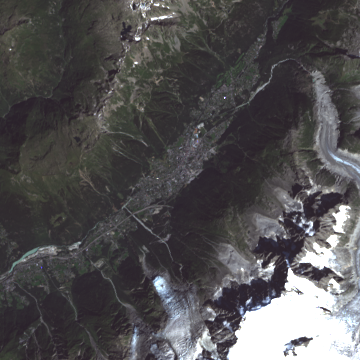
\includegraphics[scale=0.45]{images/Chamonix/08_rgb.png}
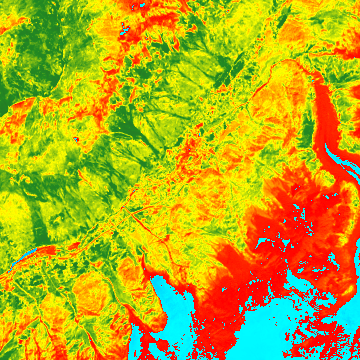
\includegraphics[scale=0.45]{images/Chamonix/08_ndvi.png}
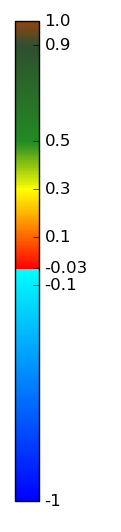
\includegraphics[scale=0.4]{images/colormap.png}
}
\begin{center}
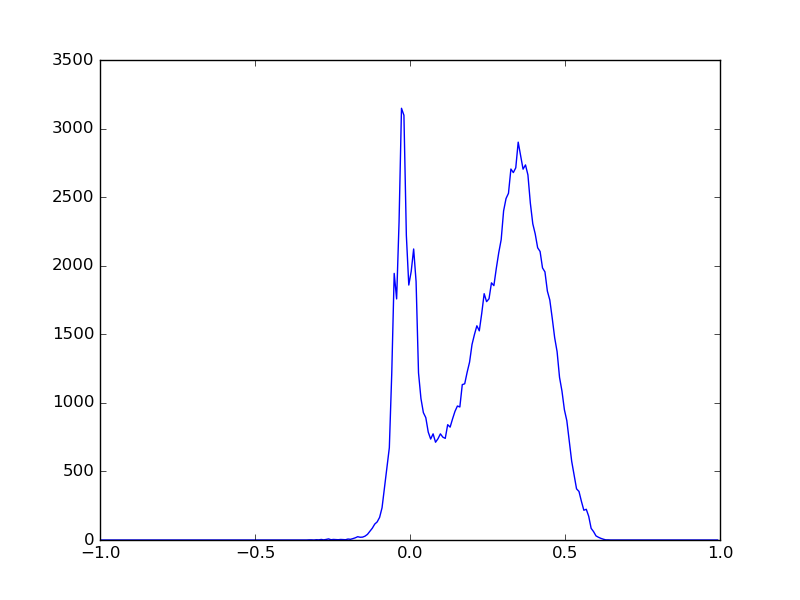
\includegraphics[scale=0.45]{images/Chamonix/08_ndvi_histo.png}
\end{center}
\caption{Image couleur, image $NDVI$ et histogramme de $NDVI$ pour la commune de $Chamonix-Mont-Blanc$ sur un périmètre de $116$km\textsuperscript{2} au mois d'$Aout$}
\label{chamonix_ndvi}
\end{figure}

La figure \ref{chamonix_ndvi} montre un $NDVI$ négatif au sud de la commune de Chamonix, ce qui correspond au glaciers du \begin{itshape}Mont-Blanc\end{itshape}\\

\clearpage 

\begin{figure}[H]
\centerline{
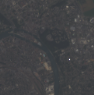
\includegraphics[scale=0.045]{images/Manaus/07_rgb.png}
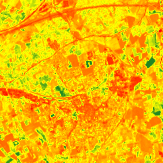
\includegraphics[scale=0.045]{images/Manaus/07_ndvi.png}
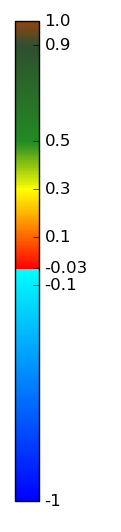
\includegraphics[scale=0.4]{images/colormap.png}
}
\begin{center}
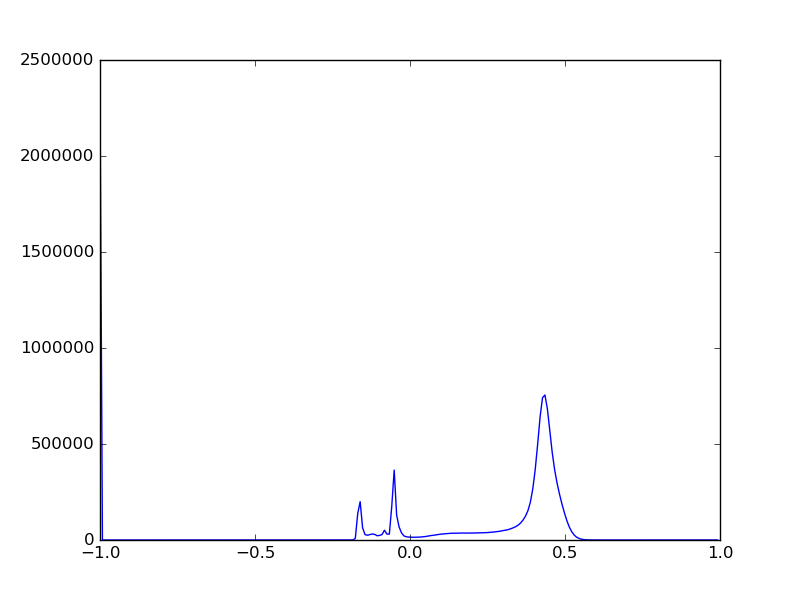
\includegraphics[scale=0.45]{images/Manaus/07_ndvi_histo.png}
\end{center}
\caption{Image couleur, image $NDVI$ et histogramme de $NDVI$ pour la ville de $Manaus$ ($Bresil$) sur un périmètre de $11000$km\textsuperscript{2} au mois de $Juillet$}
\label{manaus_ndvi}
\end{figure}

La figure \ref{manaus_ndvi} montre un $NDVI$ supérieur à $0.5$ autour de la ville de Manaus au Brésil, ce qui correspond à la végétation dense de la for\^et amazonienne. Le fleuve
du \begin{itshape}Rio Negro\end{itshape} apparait lui en négatif.\\

\clearpage

\begin{figure}[H]
\centerline{
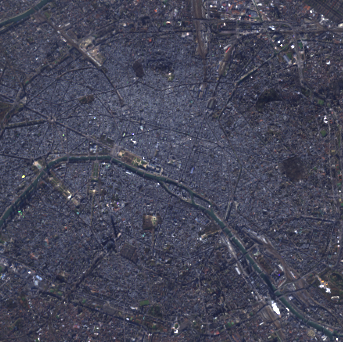
\includegraphics[scale=0.45]{images/Paris/12_rgb.png}
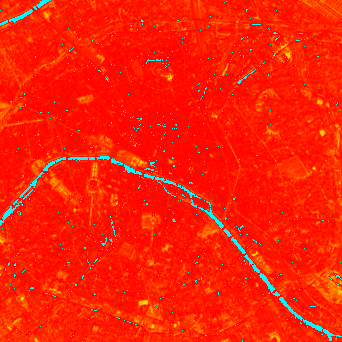
\includegraphics[scale=0.45]{images/Paris/12_ndvi.png}
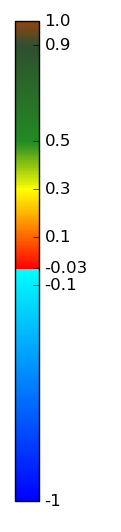
\includegraphics[scale=0.4]{images/colormap.png}
}
\begin{center}
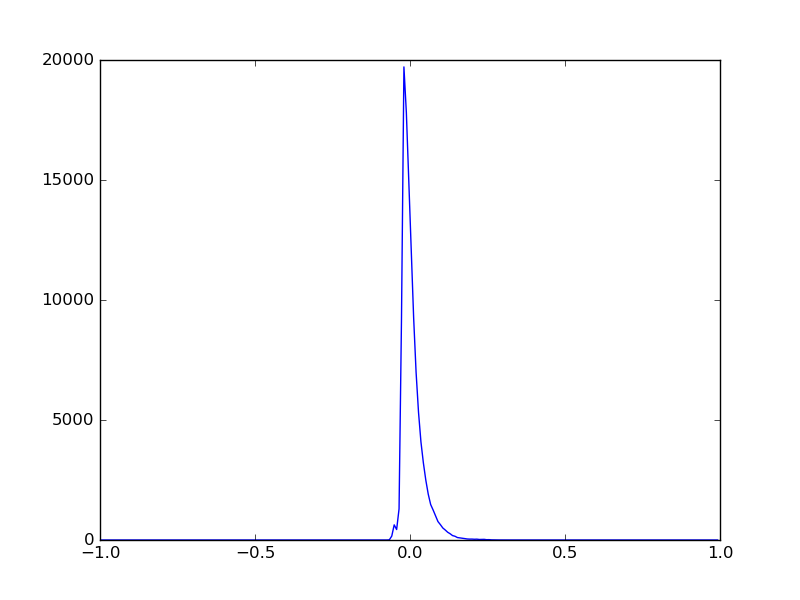
\includegraphics[scale=0.4]{images/Paris/12_ndvi_histo.png}
\end{center}
\caption{Image couleur, image $NDVI$ et histogramme de $NDVI$ pour la ville de $Paris$ sur un périmètre de $105$km\textsuperscript{2} au mois de $Decembre$}
\label{paris_ndvi}
\end{figure}

La figure \ref{paris_ndvi} montre un $NDVI$ quasi nulle donc sans végétation, comme on peut s'y attendre dans une commune urbaine telle que Paris en période hivernale.\\

\clearpage


\chapter{Evolution du NDVI au cours d'une année}

Comme vu au chapître précédent, la distribution du $NDVI$ dépend beaucoup du relief paysager (végétaux, montagnes, eau).
Ainsi, on peut légitimement se demander comment évolue cet indice en fonction des saisons.\\
Pour cela, nous allons étudier quatre types de communes selon leur paysage : urbain, plainier, montagneux, littoral.\\

\section{Pour une commune urbaine (Paris)}

La figure \ref{paris_ndvi_annee} montre l'évolution du $NDVI$ sur $10$ mois pour la ville de $Paris$. On note un étalement de la distribution 
dans les mois chauds d\^u à la vigueur des espaces verts à cette époque de l'année. Cépendant, même s'il s'éloigne de 0, le mode principal 
demeure toujours à basse fréquence ($0.05$).

\begin{figure}[H]
\centerline{
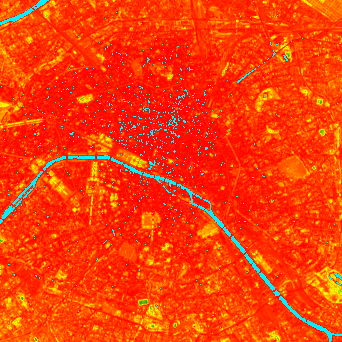
\includegraphics[scale=0.25]{images/Paris/03_ndvi.png}
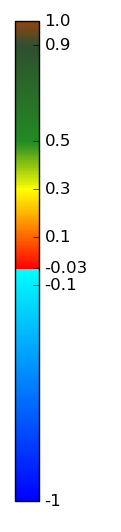
\includegraphics[scale=0.2]{images/colormap.png}
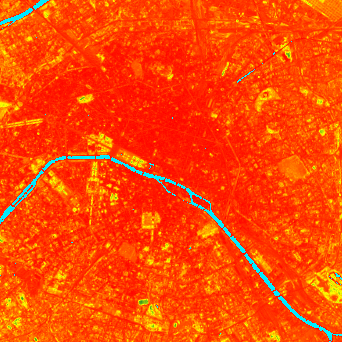
\includegraphics[scale=0.25]{images/Paris/04_ndvi.png}
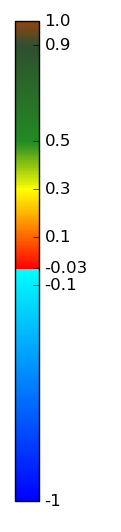
\includegraphics[scale=0.2]{images/colormap.png}
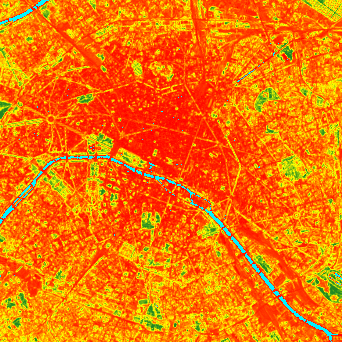
\includegraphics[scale=0.25]{images/Paris/05_ndvi.png}
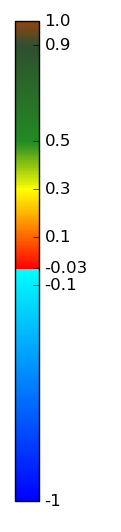
\includegraphics[scale=0.2]{images/colormap.png}
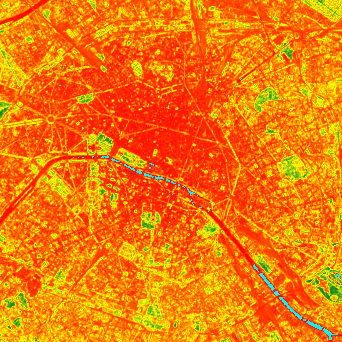
\includegraphics[scale=0.25]{images/Paris/06_ndvi.png}
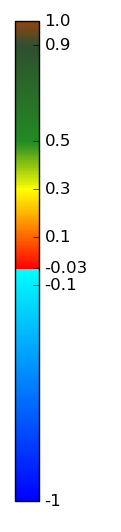
\includegraphics[scale=0.2]{images/colormap.png}
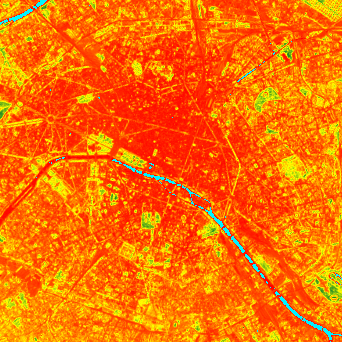
\includegraphics[scale=0.25]{images/Paris/07_ndvi.png}
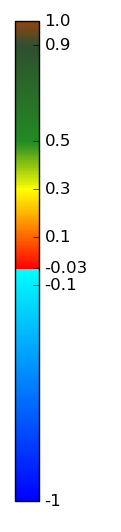
\includegraphics[scale=0.2]{images/colormap.png}
}
\centerline{
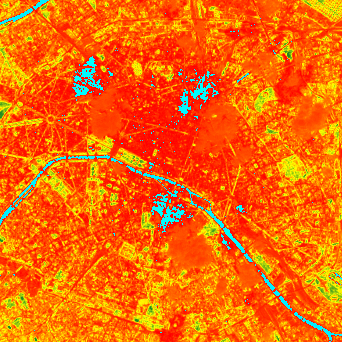
\includegraphics[scale=0.25]{images/Paris/08_ndvi.png}
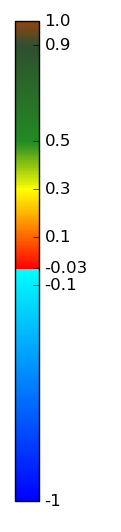
\includegraphics[scale=0.2]{images/colormap.png}
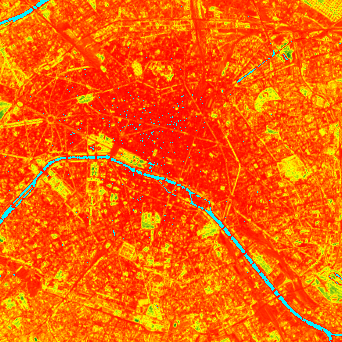
\includegraphics[scale=0.25]{images/Paris/09_ndvi.png}
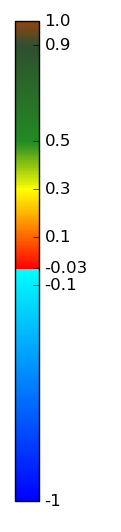
\includegraphics[scale=0.2]{images/colormap.png}
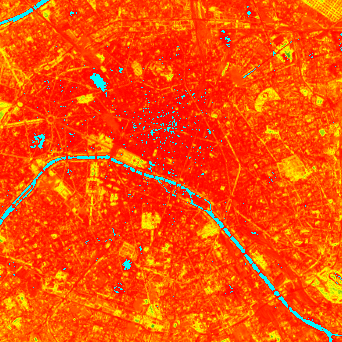
\includegraphics[scale=0.25]{images/Paris/10_ndvi.png}
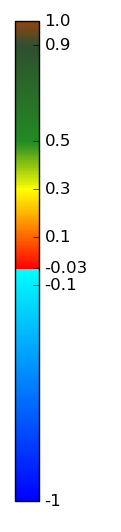
\includegraphics[scale=0.2]{images/colormap.png}
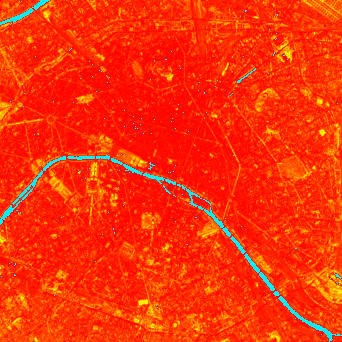
\includegraphics[scale=0.25]{images/Paris/11_ndvi.png}
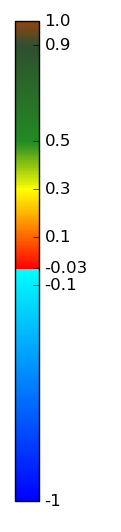
\includegraphics[scale=0.2]{images/colormap.png}
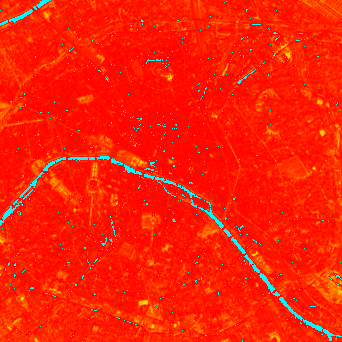
\includegraphics[scale=0.25]{images/Paris/12_ndvi.png}
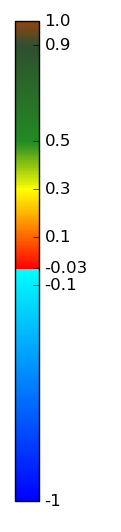
\includegraphics[scale=0.2]{images/colormap.png}
}
\begin{center}
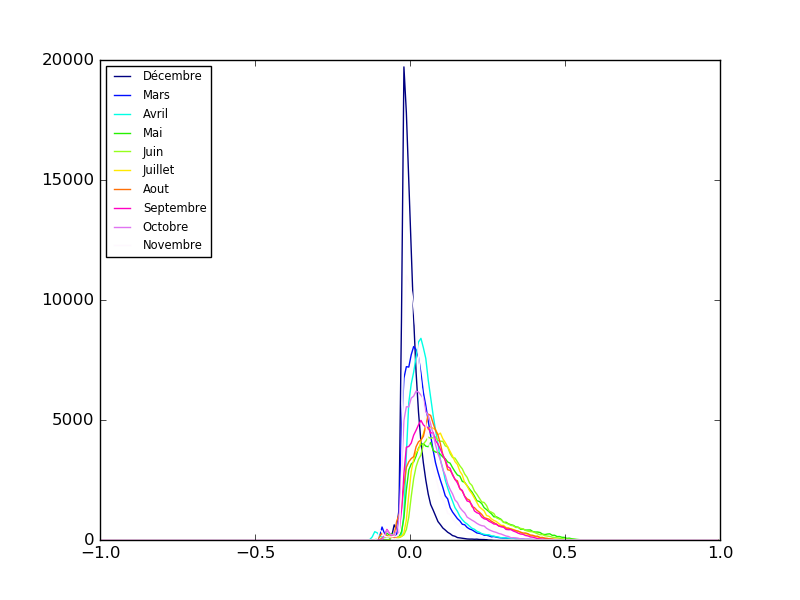
\includegraphics[scale=0.45]{images/Paris/all_ndvi_histo.png}
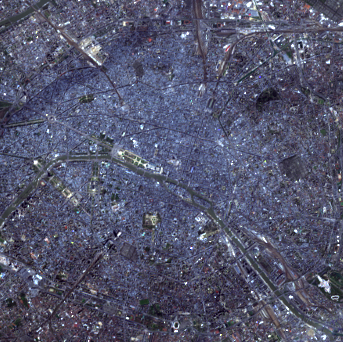
\includegraphics[scale=0.5]{images/Paris/04_rgb.png}
\end{center}
\caption{De la gauche vers la droite sur la première ligne, évolution du $NDVI$ entre $Mars$ et $Juillet$ pour la ville de $Paris$ sur un périmètre de $105$km\textsuperscript{2}.
De la gauche vers la droite sur la seconde ligne, évolution du $NDVI$ entre $Aout$ et $Decembre$ pour la ville de $Paris$ sur un périmètre de $105$km\textsuperscript{2}. 
En bas, supersposition des histogrammes de $NDVI$ pour les mois de $Mars$ à $Decembre$ et image couleur}
\label{paris_ndvi_annee}
\end{figure}

\clearpage

\section{Pour une commune plainière (Fontainebleau)}

Pour une commune plainière comme $Fontainebleau$ \ref{fontainebleau_ndvi_annee}, l'étalement de la distribution est beaucoup plus franc et déplace même
le mode principal vers les hautes fréquences ($0.5$).
 
\begin{figure}[H]
\centerline{
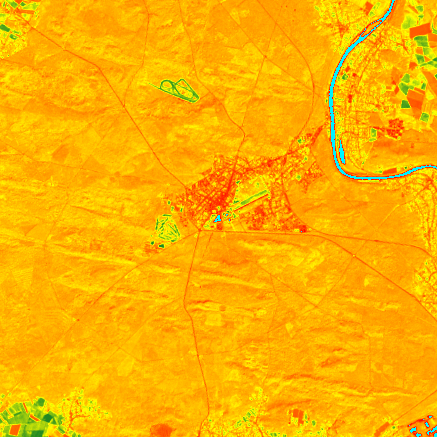
\includegraphics[scale=0.2]{images/Fontainebleau/03_ndvi.png}
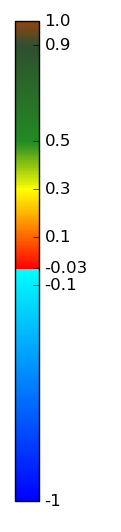
\includegraphics[scale=0.2]{images/colormap.png}
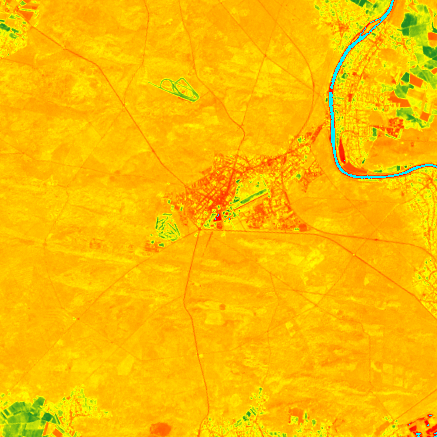
\includegraphics[scale=0.2]{images/Fontainebleau/04_ndvi.png}
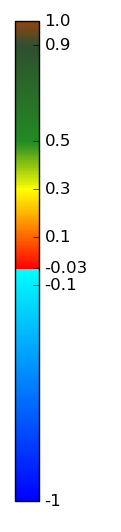
\includegraphics[scale=0.2]{images/colormap.png}
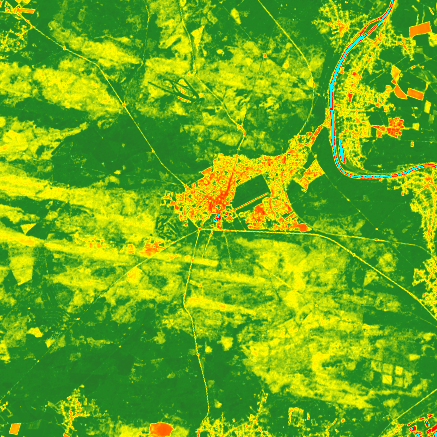
\includegraphics[scale=0.2]{images/Fontainebleau/05_ndvi.png}
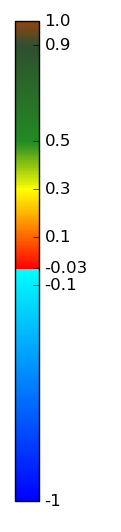
\includegraphics[scale=0.2]{images/colormap.png}
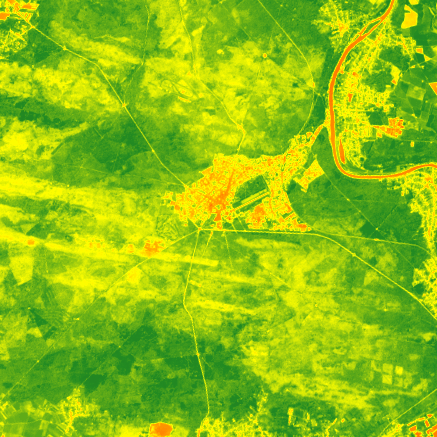
\includegraphics[scale=0.2]{images/Fontainebleau/06_ndvi.png}
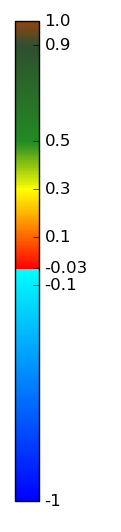
\includegraphics[scale=0.2]{images/colormap.png}
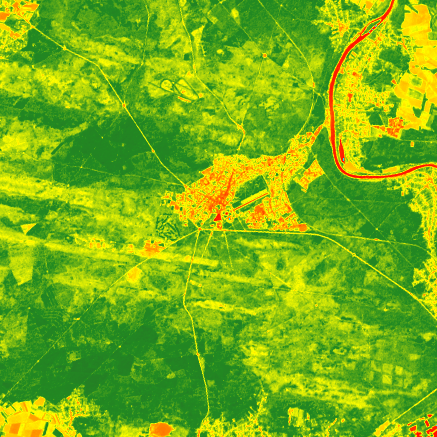
\includegraphics[scale=0.2]{images/Fontainebleau/07_ndvi.png}
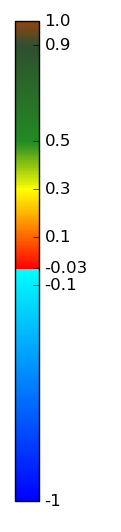
\includegraphics[scale=0.2]{images/colormap.png}
}
\centerline{
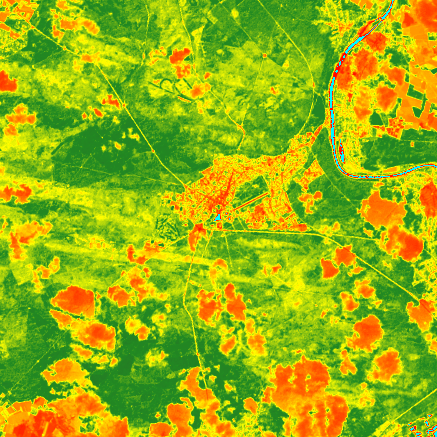
\includegraphics[scale=0.2]{images/Fontainebleau/08_ndvi.png}
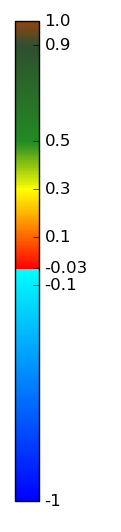
\includegraphics[scale=0.2]{images/colormap.png}
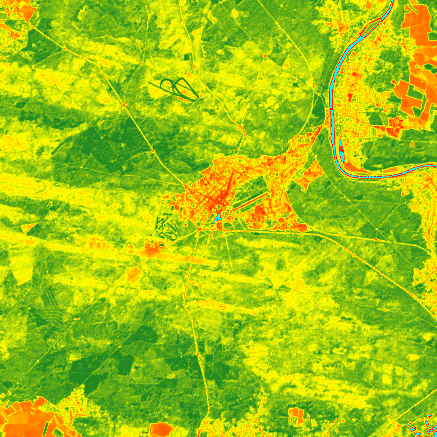
\includegraphics[scale=0.2]{images/Fontainebleau/09_ndvi.png}
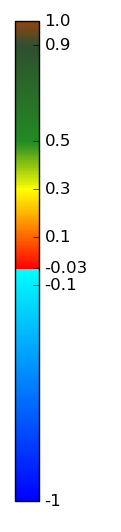
\includegraphics[scale=0.2]{images/colormap.png}
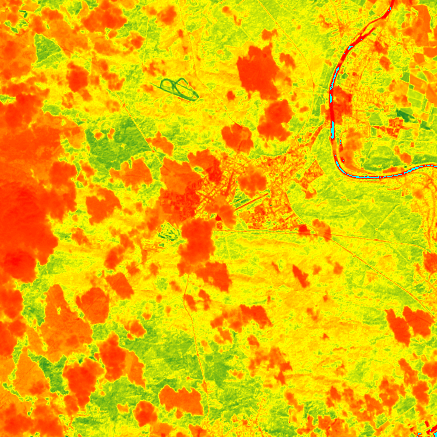
\includegraphics[scale=0.2]{images/Fontainebleau/10_ndvi.png}
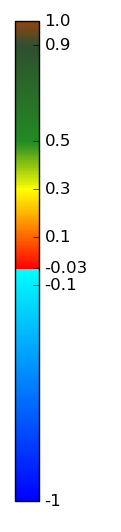
\includegraphics[scale=0.2]{images/colormap.png}
\includegraphics[scale=0.2]{images/Fontainebleau/11_ndvi.png}
\includegraphics[scale=0.2]{images/colormap.png}
\includegraphics[scale=0.2]{images/Fontainebleau/12_ndvi.png}
\includegraphics[scale=0.2]{images/colormap.png}
}
\begin{center}
\includegraphics[scale=0.45]{images/Fontainebleau/all_ndvi_histo.png}
\includegraphics[scale=0.4]{images/Fontainebleau/12_rgb.png}
\end{center}
\caption{De la gauche vers la droite sur la première ligne, évolution du $NDVI$ entre $Mars$ et $Juillet$ pour la ville de $Fontainebleau$ sur un périmètre de $172$km\textsuperscript{2}.
De la gauche vers la droite sur la seconde ligne, évolution du $NDVI$ entre $Aout$ et $Decembre$ pour la ville de $Fontainebleau$ sur un périmètre de $172$km\textsuperscript{2}. 
En bas, supersposition des histogrammes de $NDVI$ pour les mois de $Mars$ à $Decembre$ et image couleur.}
\label{fontainebleau_ndvi_annee}
\end{figure}

\clearpage

\section{Pour une commune montagneuse (Annecy)}

Pour une commune montagneuse comme Annecy \ref{annecy_ndvi_annee}, le déplacement du mode principal en saison chaude se situe à une fréquence intermédiaire ($0.2$).

\begin{figure}[H]
\centerline{
\includegraphics[scale=0.7]{images/Annecy/03_ndvi.png}
\includegraphics[scale=0.2]{images/colormap.png}
\includegraphics[scale=0.7]{images/Annecy/04_ndvi.png}
\includegraphics[scale=0.2]{images/colormap.png}
\includegraphics[scale=0.7]{images/Annecy/05_ndvi.png}
\includegraphics[scale=0.2]{images/colormap.png}
\includegraphics[scale=0.7]{images/Annecy/06_ndvi.png}
\includegraphics[scale=0.2]{images/colormap.png}
\includegraphics[scale=0.7]{images/Annecy/07_ndvi.png}
\includegraphics[scale=0.2]{images/colormap.png}
}
\centerline{
\includegraphics[scale=0.7]{images/Annecy/08_ndvi.png}
\includegraphics[scale=0.2]{images/colormap.png}
\includegraphics[scale=0.7]{images/Annecy/09_ndvi.png}
\includegraphics[scale=0.2]{images/colormap.png}
\includegraphics[scale=0.7]{images/Annecy/10_ndvi.png}
\includegraphics[scale=0.2]{images/colormap.png}
\includegraphics[scale=0.7]{images/Annecy/11_ndvi.png}
\includegraphics[scale=0.2]{images/colormap.png}
\includegraphics[scale=0.7]{images/Annecy/12_ndvi.png}
\includegraphics[scale=0.2]{images/colormap.png}
}
\begin{center}
\includegraphics[scale=0.45]{images/Annecy/all_ndvi_histo.png}
\includegraphics[scale=1.2]{images/Annecy/12_rgb.png}

\end{center}
\caption{De la gauche vers la droite sur la première ligne, évolution du $NDVI$ entre $Mars$ et $Juillet$ pour la ville de $Annecy$ sur un périmètre de $13.65$km\textsuperscript{2}.
De la gauche vers la droite sur la seconde ligne, évolution du $NDVI$ entre $Aout$ et $Decembre$ pour la ville de $Annecy$ sur un périmètre de $13.65$km\textsuperscript{2}. 
En bas, supersposition des histogrammes de $NDVI$ pour les mois de $Mars$ à $Decembre$ et image couleur.}
\label{annecy_ndvi_annee}
\end{figure}

\clearpage

\section{Pour une commune littorale (Agde)}

Pour une commune littorale comme Adge \ref{agde_ndvi_annee}, le mode principal subit une variation très légère vers les hautes fréquences en saison chaude, mais reste globalement constant dans l'année
autour de $0.25$.

\begin{figure}[H]
\centerline{
\includegraphics[scale=0.4]{images/Agde/03_ndvi.png}
\includegraphics[scale=0.2]{images/colormap.png}
\includegraphics[scale=0.4]{images/Agde/04_ndvi.png}
\includegraphics[scale=0.2]{images/colormap.png}
\includegraphics[scale=0.4]{images/Agde/05_ndvi.png}
\includegraphics[scale=0.2]{images/colormap.png}
\includegraphics[scale=0.4]{images/Agde/06_ndvi.png}
\includegraphics[scale=0.2]{images/colormap.png}
\includegraphics[scale=0.4]{images/Agde/07_ndvi.png}
\includegraphics[scale=0.2]{images/colormap.png}
}
\centerline{
\includegraphics[scale=0.4]{images/Agde/08_ndvi.png}
\includegraphics[scale=0.2]{images/colormap.png}
\includegraphics[scale=0.4]{images/Agde/09_ndvi.png}
\includegraphics[scale=0.2]{images/colormap.png}
\includegraphics[scale=0.4]{images/Agde/10_ndvi.png}
\includegraphics[scale=0.2]{images/colormap.png}
\includegraphics[scale=0.4]{images/Agde/11_ndvi.png}
\includegraphics[scale=0.2]{images/colormap.png}
\includegraphics[scale=0.4]{images/Agde/12_ndvi.png}
\includegraphics[scale=0.2]{images/colormap.png}
}
\begin{center}
\includegraphics[scale=0.45]{images/Agde/all_ndvi_histo.png}
\includegraphics[scale=0.7]{images/Agde/12_rgb.png}

\end{center}
\caption{De la gauche vers la droite sur la première ligne, évolution du $NDVI$ entre $Mars$ et $Juillet$ pour la ville de $Adge$ sur un périmètre de $50.9$km\textsuperscript{2}.
De la gauche vers la droite sur la seconde ligne, évolution du $NDVI$ entre $Aout$ et $Decembre$ pour la ville de $Adge$ sur un périmètre de $50.9$km\textsuperscript{2}. 
En bas, supersposition des histogrammes de $NDVI$ pour les mois de $Mars$ à $Decembre$ et image couleur}
\label{agde_ndvi_annee}
\end{figure}
\clearpage

Ainsi, nous avons pu mettre en évidence divers comportements de l'indice en fonction des saisons et du paysage. On note que la distribution au mois de Juin-Juillet est 
très dispersée. En effet, la végétation des zones faiblement urbaines (litoral, plaine, montagne) n'est pas toujours visible en dehors de la période estivale, hors c'est la
végétation qui doit pouvoir nous renseigner sur la densité d'une zone donnée.\\
Dans la partie qui suit, nous allons définir plusieurs catégories de commune liées à la densité de population et observer leur $NDVI$ pour la période estivale.\\

\chapter{Evolution du NDVI en fonction de la densité de population}

L'INSEE définit quatre types de communes en fonction de la densité de population. Nous reprenons ci-après la nomenclature telle que définie sur le
site de l'organisme public \cite{insee}:\\

\begin{quotation}
\begin{itshape}
La nouvelle typologie de l’Insee s’inspire de la classification européenne urbain-rural conçue à partir des données carroyées de population. 
Elle permet de définir 3 types d’espace :\\

\begin{description}
\item[les communes densément peuplées :] dont la densité de population au carreau est d’au moins 1 500 habitants par km\textsuperscript{2} 
et qui comptabilisent un minimum de 50 000 habitants ;

\item[Les communes de densité intermédiaire :] les carreaux contigus ayant une densité de population d’au moins 300 habitants par km\textsuperscript{2} 
et un minimum de 5 000 habitants ;

\item[Les communes peu denses :] les carreaux contigus ayant une densité de population de moins de 300 habitants par km\textsuperscript{2} 
et moins de 5 000 habitants.
Avec cette typologie, 90 \% des communes françaises sont « rurales ». L’Insee rajoute alors un 4e degré en partant de la «maille rurale » (peu dense) :

\item[les communes très peu denses :] carreaux de densité de population d’au moins 25 habitants par km\textsuperscript{2} et moins de 300 habitants
\end{description}
\end{itshape}
\end{quotation}

Pour chacune de ces quatres catégories, nous avons choisis trois communes \ref{cat1},\ref{cat2},\ref{cat3},\ref{cat4}:\\

\clearpage

\begin{table}
\begin{center}
\begin{adjustbox}{max width=\textwidth}
\begin{tabular}{|c|c|c|}
\hline
\multicolumn{3}{c|}{\begin{bf}communes densément peuplées\end{bf}} \\
\hline 
nom & densité (habs/km\textsuperscript{2}) & nombre d'habitants \\
\hline 
Lyon & 10117 & 474900\\
\hline 
Montpellier & 4524 & 253000 \\
\hline 
Amiens & 2689 & 134400 \\
\hline
\end{tabular}
\end{adjustbox}
\end{center}
\caption{Trois communes densément peuplées : $Lyon$, $Montpellier$, $Amiens$}
\label{cat1}
\end{table}

\begin{table}
\begin{center}
\begin{adjustbox}{max width=\textwidth}
\begin{tabular}{|c|c|c|}
\hline
\multicolumn{3}{c|}{\begin{bf}communes de densité intermédiaire\end{bf}} \\
\hline 
nom & densité (habs/km\textsuperscript{2}) & nombre d'habitants \\
\hline 
Abbeville & 914 & 24100\\
\hline 
Louvres & 824 & 9000 \\
\hline 
Limours & 453 & 6400 \\
\hline
\end{tabular}
\end{adjustbox}
\end{center}
\caption{Trois communes de densité intermédiaire : $Abbeville$, $Louvres$, $Limours$}
\label{cat2}
\end{table}

\begin{table}
\begin{center}
\begin{adjustbox}{max width=\textwidth}
\begin{tabular}{|c|c|c|}
\hline
\multicolumn{3}{c|}{\begin{bf}communes peu denses\end{bf}} \\
\hline 
nom & densité (habs/km\textsuperscript{2}) & nombre d'habitants \\
\hline 
Roissy-en-France & 195 & 2500\\
\hline 
Fontenay-en-Parisis & 176 & 2000 \\
\hline 
Malay-le-Grand & 69 & 1600 \\
\hline
\end{tabular}
\end{adjustbox}
\end{center}
\caption{Trois communes peu denses : $Roissy-en-France$, $Fontenay-en-Parisis$, $Malay-le-Grand$}
\label{cat3}
\end{table}

\begin{table}
\begin{center}
\begin{adjustbox}{max width=\textwidth}
\begin{tabular}{|c|c|c|}
\hline
\multicolumn{3}{c|}{\begin{bf}communes très peu denses\end{bf}} \\
\hline 
nom & densité (habs/km\textsuperscript{2}) & nombre d'habitants \\
\hline 
Brignancourt & 66 & 200\\
\hline 
Omiécourt & 43 & 200 \\
\hline 
Marieux & 27 & 100 \\
\hline
\end{tabular}
\end{adjustbox}
\end{center}
\caption{Trois communes très peu denses : $Brignancourt$, $Omiecourt$, $Marieux$}
\label{cat4}
\end{table}

\clearpage

La figure \ref{ndvi_categorie} montre la superposition des courbes de $NDVI$ au mois de $Juillet$ pour chacune des communes de chaque catégorie :\\
\begin{figure}[H]
\centerline{
\includegraphics[scale=0.5]{images/ndvi_categorie.png}
}
\caption{Superposition des courbes de $NDVI$ pour les communes densément peuplées (rouge), les communes de densité intermédiaire (bleu),
les communes peu denses (jaune) ainsi que les communes très peu denses (vert)}
\label{ndvi_categorie}
\end{figure}
\clearpage

Nous observons donc que les communes les plus denses sont caractérisés par un spectre d'amplitude fort et distribué vers les basses fréquences. A mesure 
qu'on se déplace vers les communes les moins denses, on constate une diminution d'amplitude et un déplacement de la distribution de $NDVI$ vers les
hautes fréquences.\\
Les figures \ref{ndvi_cat1},\ref{ndvi_cat2},\ref{ndvi_cat3} et \ref{ndvi_cat4} présentent les images de $NDVI$ pour les communes de chaque catégorie.\\ 

\begin{figure}[H]
\centerline{
\includegraphics[scale=0.6]{images/Lyon/07_rgb.png}
\includegraphics[scale=0.6]{images/Lyon/07_ndvi.png}
\includegraphics[scale=0.3]{images/colormap.png}
}
\centerline{
\includegraphics[scale=0.6]{images/Montpellier/07_rgb.png}
\includegraphics[scale=0.6]{images/Montpellier/07_ndvi.png}
\includegraphics[scale=0.3]{images/colormap.png}
}
\centerline{
\includegraphics[scale=0.6]{images/Amiens/07_rgb.png}
\includegraphics[scale=0.6]{images/Amiens/07_ndvi.png}
\includegraphics[scale=0.3]{images/colormap.png}
}
\caption{Image $NDVI$ et image couleur au mois de $Juillet$ pour les trois communes densément peuplées, de haut en bas respectivement :
$Lyon$ ($10117$ habs/km\textsuperscript{2}),
$Montpellier$ ($4524$ habs/km\textsuperscript{2}),
$Amiens$ ($2689$ habs/km\textsuperscript{2}),
}
\label{ndvi_cat1}
\end{figure}
\clearpage

\begin{figure}[H]
\centerline{
\includegraphics[scale=0.9]{images/Abbeville/07_rgb.png}
\includegraphics[scale=0.9]{images/Abbeville/07_ndvi.png}
\includegraphics[scale=0.3]{images/colormap.png}
}
\centerline{
\includegraphics[scale=0.9]{images/Louvres/07_rgb.png}
\includegraphics[scale=0.9]{images/Louvres/07_ndvi.png}
\includegraphics[scale=0.3]{images/colormap.png}
}
\centerline{
\includegraphics[scale=0.9]{images/Limours/07_rgb.png}
\includegraphics[scale=0.9]{images/Limours/07_ndvi.png}
\includegraphics[scale=0.3]{images/colormap.png}
}
\caption{Image $NDVI$ et image couleur au mois de $Juillet$ pour les trois communes de densité intermédiaire, de haut en bas respectivement :
$Abbeville$ ($914$ habs/km\textsuperscript{2}),
$Louvres$ ($824$ habs/km\textsuperscript{2}),
$Limours$ ($453$ habs/km\textsuperscript{2}),
}
\label{ndvi_cat2}
\end{figure}
\clearpage

\begin{figure}[H]
\centerline{
\includegraphics[scale=1.1]{images/Roissy-en-France/07_rgb.png}
\includegraphics[scale=1.1]{images/Roissy-en-France/07_ndvi.png}
\includegraphics[scale=0.3]{images/colormap.png}
}
\centerline{
\includegraphics[scale=1.1]{images/Fontenay-en-Parisis/07_rgb.png}
\includegraphics[scale=1.1]{images/Fontenay-en-Parisis/07_ndvi.png}
\includegraphics[scale=0.3]{images/colormap.png}
}
\centerline{
\includegraphics[scale=1.1]{images/Malay-le-Grand/07_rgb.png}
\includegraphics[scale=1.1]{images/Malay-le-Grand/07_ndvi.png}
\includegraphics[scale=0.3]{images/colormap.png}
}
\caption{Image $NDVI$ et image couleur au mois de $Juillet$ pour les trois communes peu denses, de haut en bas respectivement :
$Roissy-en-France$ ($195$ habs/km\textsuperscript{2}),
$Fontenay-en-Parisis$ ($176$ habs/km\textsuperscript{2}),
$Malay-le-Grand$ ($63$ habs/km\textsuperscript{2}),
}
\label{ndvi_cat3}
\end{figure}
\clearpage

\begin{figure}[H]
\centerline{
\includegraphics[scale=1.5]{images/Brignancourt/07_rgb.png}
\includegraphics[scale=1.5]{images/Brignancourt/07_ndvi.png}
\includegraphics[scale=0.3]{images/colormap.png}
}
\centerline{
\includegraphics[scale=1.5]{images/Omiecourt/07_rgb.png}
\includegraphics[scale=1.5]{images/Omiecourt/07_ndvi.png}
\includegraphics[scale=0.3]{images/colormap.png}
}
\centerline{
\includegraphics[scale=1.5]{images/Marieux/07_rgb.png}
\includegraphics[scale=1.5]{images/Marieux/07_ndvi.png}
\includegraphics[scale=0.3]{images/colormap.png}
}
\caption{Image $NDVI$ et image couleur au mois de $Juillet$ pour les trois communes peu denses, de haut en bas respectivement :
$Brignancourt$ ($66$ habs/km\textsuperscript{2}),
$Omiecourt$ ($43$ habs/km\textsuperscript{2}),
$Marieux$ ($27$ habs/km\textsuperscript{2}),
}
\label{ndvi_cat4}
\end{figure}
\clearpage


\clearpage
%Paris 21288
%Versailles 3289
%Fontainebleau 89
%Melun 4924
%Albertville 1076
%Annecy 3690
%Chambéry 2731
%Chamonix-Mont-Blanc 76
%Bourg-en-Bresse 1680
%Lyon 10117
%Thonon-les-Bains 2092
%Montpellier 4524
\backmatter

\listoftables

\listoffigures

\bibliographystyle{alpha}
\bibliography{biblio}

\end{document}